\let\negmedspace\undefined
\let\negthickspace\undefined
\documentclass[journal]{IEEEtran}
\usepackage[a5paper, margin=10mm, onecolumn]{geometry}
%\usepackage{lmodern} % Ensure lmodern is loaded for pdflatex
\usepackage{tfrupee} % Include tfrupee package

\setlength{\headheight}{1cm} % Set the height of the header box
\setlength{\headsep}{0mm}     % Set the distance between the header box and the top of the text

\usepackage{gvv-book}
\usepackage{gvv}
\usepackage{cite}
\usepackage{amsmath,amssymb,amsfonts,amsthm}
\usepackage{algorithmic}
\usepackage{graphicx}
\usepackage{textcomp}
\usepackage{xcolor}
\usepackage{txfonts}
\usepackage{listings}
\usepackage{enumitem}
\usepackage{mathtools}
\usepackage{gensymb}
\usepackage{comment}
\usepackage[breaklinks=true]{hyperref}
\usepackage{tkz-euclide} 
\usepackage{listings}
% \usepackage{gvv}                                        
\def\inputGnumericTable{}                                 
\usepackage[latin1]{inputenc}                                
\usepackage{color}                                            
\usepackage{array}                                            
\usepackage{longtable}                                       
\usepackage{calc}                                             
\usepackage{multirow}                                         
\usepackage{hhline}                                           
\usepackage{ifthen}                                           
\usepackage{lscape}
\begin{document}

\bibliographystyle{IEEEtran}
\vspace{3cm}

\title{3.3.20}
\author{EE24BTECH11011-B.PRANAY KUMAR
}
 \maketitle
% \newpage
% \bigskip
{\let\newpage\relax\maketitle}

\renewcommand{\thefigure}{\theenumi}
\renewcommand{\thetable}{\theenumi}
\setlength{\intextsep}{10pt} % Space between text and floats


\numberwithin{equation}{enumi}
\numberwithin{figure}{enumi}
\renewcommand{\thetable}{\theenumi}



\textbf{Question}:\\
Draw a triangle $PQR$ in which $QR = 3$ cm, $QP - PR = 6$ cm, and $\angle PQR = 45\degree$.\\

\solution

For triangle $PQR$ with $QR = 3$ cm, $QP - PR = 6$ cm, and $\angle PQR = 45\degree$.\\
Using law of cosines:
\begin{align}
    QP^2 = QR^2 + PR^2 - 2(QR) (PR) \angle PQR 
\end{align}
\begin{align}
    K (QP+PR) = QR^2 - 2 (QR) (PR) \angle PQR 
\end{align}
Where,
\begin{align}
    K = QP-PR
\end{align}

\begin{align}
    \myvec{1 & 1 \\ 1 & -1} \myvec{QP\\ PR} &= \myvec{QR^2 - 2(QR)(PR) \cos PQR \\ K} \\
    \myvec{QP \\ PR} &= \frac{1}{K} \myvec{1 & 1 \\ 1 & -1} \myvec{QR^2 - 2(QR)(PR) \cos PQR \\ K} \\
    \because \myvec{1 & 1 \\ 1 & -1} \myvec{1 & 1 \\ 1 & -1} &= 2I
\end{align}



\begin{align}
    PR = \frac{1}{2(1+\frac{2(QR)\ COS \angle(PQR)}{K})} \Vec{e}^\top \myvec{1 &1\\ 1 & -1} \myvec{\frac{QR^2}{K}\\ K}
\end{align}
The coordinates of $\triangle PQR$ are
\begin{align}
    \vec P = PR \myvec{Cos\angle PQR\\ Sin \angle PQR} , \vec Q = \myvec{0 \\ 0} , \vec R = \myvec{QR \\ 0}
\end{align}
substituting $QR = 3$ and $K=-6$ in $(0.7)$
\begin{align}
    QR = \frac{45}{6(2-\sqrt{2})}\\
    QR = 11.803300859
\end{align}
Hence;
\begin{align}
    \vec{P} = \frac{11.803300859}{\sqrt{2}} \myvec{1 \\ 1}, \\
    \vec{Q} = \myvec{0 \\ 0}, \\
    \vec{R} = \myvec{3 \\ 0}.
\end{align}
\begin{figure}[h!]
   \centering
   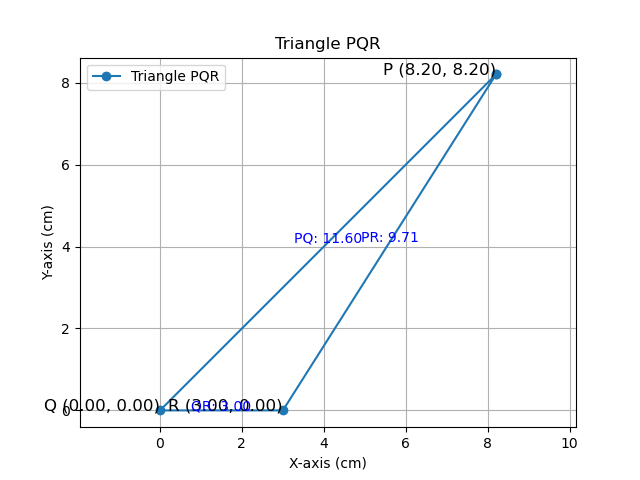
\includegraphics[width=0.7\linewidth]{figs/triangle_plot.png}
   \caption{Triangle $PQR$}
\end{figure}

\end{document}


